% !TeX encoding = UTF-8
% !TeX program = xelatex
% !TeX spellcheck = en_US

\documentclass[a4paper]{ltxdoc}
\usepackage{amsmath}
\usepackage[UTF8]{ctex}
\usepackage{unicode-math}
\usepackage{caption}
\usepackage{booktabs}
\usepackage{xcolor}
\usepackage{array}
\usepackage{listings}
\usepackage[perpage]{footmisc}
\usepackage{hypdoc}
\usepackage{geometry}
\usepackage{endnotes}
\usepackage{graphicx}
\usepackage{multirow}
\usepackage{longtable}
% \usepackage[multiple]{endnotes}
\usepackage{multicol}
\usepackage{blindtext}
\geometry{a4paper, scale=0.85}
\newenvironment{Figure}
  {\par\medskip\noindent\minipage{\linewidth}}
  {\endminipage\par\medskip}


\title {实验报告\\拉伸法测量钢丝的杨氏模量}
\author {少年班学院\\马天开 PB21000030}
\date {\today}


\begin{document}
\begin{multicols}{2}
    \maketitle

    \section{实验背景及目的}

    实验背景:杨氏模量是描述刚性材料在弹性限度内材料拉伸(或压缩)性能的物理量,仅取决于材料本身的性质,与尺寸、形状、外力大小(弹性限度内)无关。更具体地说,杨氏模量越大,物体约不容易发生形变。

    \begin{equation}
        E = (F/S) / (\Delta L / L) = FL/S\Delta L
        \notag
    \end{equation}

    实验目的:利用光杠杆放大法测量形变量,利用线性回归给出钢丝杨氏模量的计算值。

    \section{实验原理}

    实验装置下图所示:

    \begin{Figure}
        \centering
        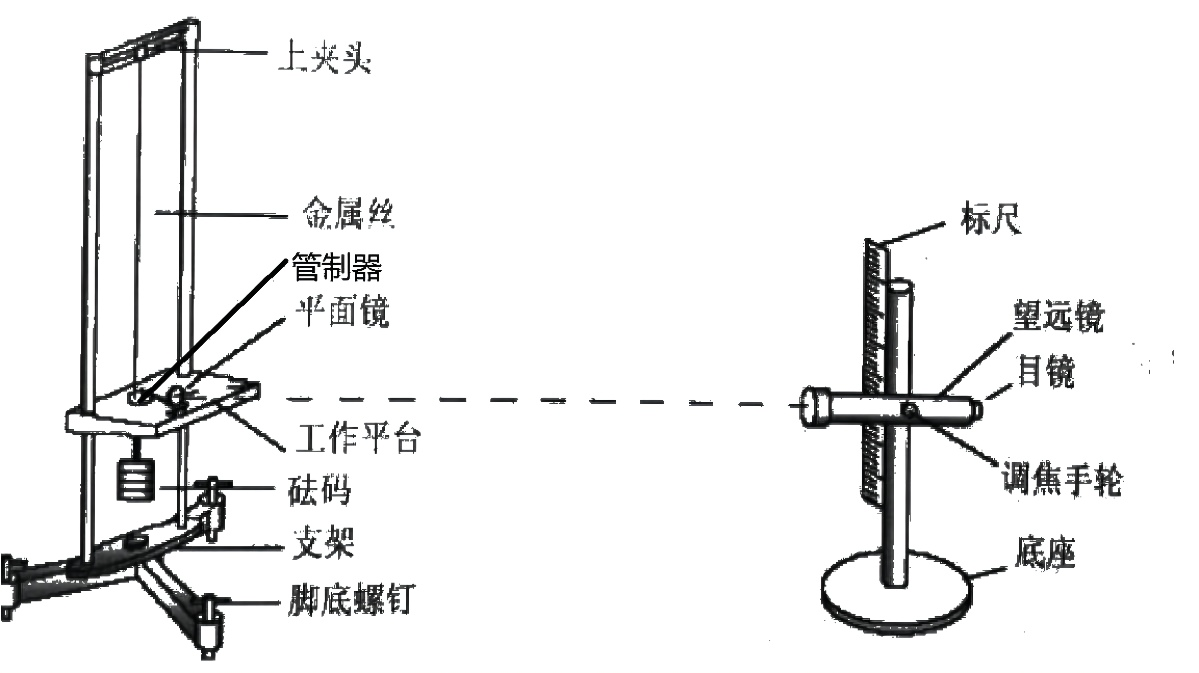
\includegraphics[width=\linewidth]{img/1.png}
        % \caption{示意图}
    \end{Figure}

    其中金属丝的长度约为$1m$,上端加紧在支架顶部。金属丝的下部连接了一个管制器,管制器连有一个法玛托盘。

    通过调节砝码盘上法码的数量可以调整受力。

    在望远镜的像中读数可以得到$\Delta L$,从而计算出杨氏模量。

    \section{实验过程}

    \begin{itemize}
        \item 调节仪器:保持支架、工作平台水平;调整平台上下位置,与管制器顶部齐平。
        \item 调节光杠杆的刀口嵌入管制器平台对应位置
        \item 调节望远镜、直尺、光杆杆之间的相对位置,调整望远镜目镜及物镜焦距,使标尺清晰。
        \item 在砝码托上逐次曾加砝码,记录每增加一个砝码后标尺像的读数$b_i$,然后再逐次减去,记录对应的读数$b_i$,取两次记录的平均值。
        \item 测量金属丝长度$L$,平面镜与标尺之间的距离$D$,光杠杆的臂长$l$,金属丝的直径$d$
    \end{itemize}

    \section{实验数据}

    $b_i$的读数:

    \smallskip

    \begin{tabular}{|c|c|c|c|}
        \hline \textbf{砝码数} & \textbf{读数 1} & \textbf{读数 2} & \textbf{平均值} \\
        \hline $m_0$           & 2.67            & 2.60            & 2.635           \\
        \hline $m_0 + m$       & 4.00            & 4.06            & 4.03            \\
        \hline $m_0 + 2m$      & 5.53            & 5.71            & 5.62            \\
        \hline $m_0 + 3m$      & 6.92            & 7.45            & 7.185           \\
        \hline $m_0 + 4m$      & 8.58            & 9.23            & 8.905           \\
        \hline $m_0 + 5m$      & 9.88            & 10.65           & 10.265          \\
        \hline $m_0 + 6m$      & 11.40           & 12.41           & 11.905          \\
        \hline $m_0 + 7m$      & 13.30           & 13.60           & 13.45           \\\hline
    \end{tabular}

    \smallskip

    螺旋测微器零示数:$-0.010cm$

    \smallskip

    直径$d$的读数:$0.267cm,0.271cm,0.273cm$

    \smallskip

    金属丝的长度$L$:$81.90cm,81.82cm,81.79cm$

    \smallskip

    距离$D$:$157.42cm,157.31cm,157.53cm$

    \smallskip

    光杠杆的长度$l$:$7.02cm,7.05cm,7.03cm$

    \smallskip

    单个砝码重量:$0.5kg$(标称值)

    \section{数据处理}

    由以上数据,首先计算出各项的平均值分别为:

    \begin{equation}
        \left\{
        \begin{aligned}
            \bar d & = 0.280cm  \\
            \bar L & = 81.84cm  \\
            \bar D & = 157.42cm \\
            \bar l & = 7.03cm   \\
        \end{aligned}
        \right.
        \notag
    \end{equation}

    同时,由于测量次数均为$n=3$,可以计算出各组的A类不确定度分别为:

    \begin{equation}
        \left\{
        \begin{aligned}
            u_{A(d)} & = 0.00178cm \\
            u_{A(L)} & = 0.0329cm  \\
            u_{A(D)} & = 0.0635cm  \\
            u_{A(l)} & = 0.00913cm \\
        \end{aligned}
        \right.
        \notag
    \end{equation}

    钢丝的长度$L$,取置信区间0.997:

    \begin{equation}
        \begin{aligned}
             & \Delta L             = 1.2mm,C=3 \\
             & \therefore u_{B(l)}  = 0.0004m   \\
        \end{aligned}
        \notag
    \end{equation}

    类似的,可以计算出:

    \begin{equation}
        \left\{
        \begin{aligned}
            u_{A(d)} & = 0.00013cm \\
            u_{A(L)} & = 0.04cm    \\
            u_{A(D)} & = 0.04cm    \\
            u_{A(l)} & = 0.04cm    \\
        \end{aligned}
        \right.
        \notag
    \end{equation}

    所以,最后计算各测量值的展伸不确定度为:

    \begin{equation}
        \left\{
        \begin{aligned}
            U_{d} & = 0.00178cm \\
            U_{L} & = 0.0331cm  \\
            U_{D} & = 0.075cm   \\
            U_{l} & = 0.041cm   \\
        \end{aligned}
        \right.
        \notag
    \end{equation}

    另外计算受力$F_i$,取重力加速度$g=9.79m/s^2$,做$b_i \sim F_i$的图像:

    \begin{Figure}
        \centering
        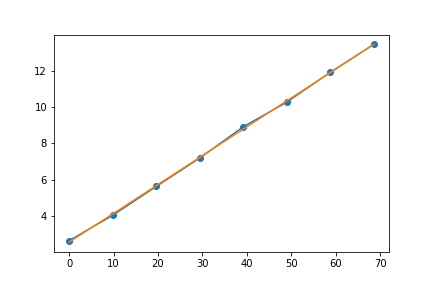
\includegraphics[width=\linewidth]{img/2.png}
    \end{Figure}

    回归直线:$b_i =0.159 * F_i + 2.552$

    由公式$E=\dfrac{2DLF}{Slb}$,得到:

    \smallskip

    $b_i = \dfrac{2DLF_i}{SLE} = \dfrac{8DLF_i}{\pi d^2 lE}$

    \smallskip

    $\therefore E = \dfrac{8DL}{\pi d^2 l k} = 1.9253 \times 10^{11} N / m^2 $

    \smallskip

    同时,斜率的标准差$S_k$满足:

    \smallskip

    $S_k = k\cdot \sqrt{\dfrac{\dfrac {1} {R^2} -1}{n-2}} = 0.796 \times 10^{-5}$

    \smallskip

    综上,$E$的不确定度满足:

    \begin{equation}
        \begin{aligned}
            \dfrac{U_E} {E} & = \sqrt{4(\dfrac{U_d}{d})^2 + (\dfrac{U_l}{l})^2 + (\dfrac{U_L}{L})^2 + (\dfrac{U_D}{D})^2 + (\dfrac {t_p S_k} {k})^2} \\
            =               & 0.014                                                                                                                  \\
        \end{aligned}
        \notag
    \end{equation}

    $\therefore \Delta E = 0.027 \times 10 ^{11} N / m^2$

    \section{实验结论}

    $E = 1.9253 \pm 0.027 \times 10^{11} N /m^2 (P =0.997)$,与公认值$2.0\times 10^11 N/m^2$的相对误差在$\omega = 3.7\%$,符合预期。

    \section{思考题}

    \begin{itemize}
        \item 利用光杠杆把测微小长度$\Delta L$ 变成测 $b$,光杠杆的放大率为 $2D/L$,根据此式能否以增加 $D$减小 $l$ 来提高放大率,这样做有无好处?有无限度?应怎样考虑这个问题?

              可以提高放大率,但受限于标尺量程,有可能会导致实验测量的数据点减少,从而影响精度。
        \item 实验中,各个长度量用不同的仪器来测量是怎样考虑的,为什么?

              要综合考虑待测物体的长度是否超出量程范围,并且考虑精度来尽可能降低不确定度。
    \end{itemize}
\end{multicols}
\end{document}